\documentclass[ngerman, a4paper]{scrartcl}

\usepackage{graphicx}
\usepackage[bottom=3cm]{geometry}
\usepackage{babel}
\usepackage{enumitem}
\usepackage[format=plain, indention=0em]{caption} % Make multiline captions not ugly.
\usepackage{hyperref, cleveref-forward}

\usepackage{todonotes}
\setuptodonotes{inline}

\title{Hier steht ein toller Titel}
\author{Autor}
\date{September 2026}

\newcommand{\coc}{\emph{Cycle of Cinder}}

\begin{document}

\maketitle

\tableofcontents % Weiß nicht, ob das drinnen bleiben sollte, aber es hilft zumindest beim Planen.

\section{Einleitung}

\section{Finanzplan}
\todo{Oder so, keine Ahnung}

\todo{
    Ich glaube, noch ein paar mehr Bilder wären nicht verkehrt, um zum Einen die langen Textblöcke aufzubrechen, und zum anderen stärker zu zeigen, dass es nicht nur ein leeres Konzept ist sondern schon einiges existiert.
}

\section{Cycle of Cinder}
    \todo{
    Die Einleitung muss definitiv überarbeitet werden. Tendenziell sollte sie eher kürzer werden als länger.
    Ich sehe 2 sinnvolle Möglichkeiten zum Strukturieren:
    1. Ein kurzer Abschnitt zu jedem der folgenden Themen (also Core Loop, Roguelite, Spielererfahrung, Thematische Einbettung, Projektplan).
    	- Die können jeweils sehr kurz sein, bei manchen reicht ein einzelner Paragraph!
    2. Unterabschnitt pro Spielmodus. Aktuell hat der Roguelite effektive 3 bzw. 4 Abschnitte.
}

\coc\ ist ein digitales Singleplayer-Kartenspiel und Roguelite, dessen Kern ein von uns neu entwickelter Gameplay Loop ist.
Statt auf einem etablierten Kartenkampf- oder Deckbuilding-System aufzubauen, basiert das Spiel auf einem eigenständigen, puzzle-artigen Spielprinzip:
Die einzelnen Level, sogenannte `Encounter', stellen jeweils strategische Problemsituationen dar, die mit den verfügbaren Karten, Ressourcen und Fähigkeiten gelöst werden müssen.
Dieser neuartige Encounter-basierte Gameplay Loop bildet das zentrale Fundament des gesamten Spiels und soll ein Spielgefühl schaffen, das sich deutlich von bestehenden digitalen Kartenspielen und Roguelites unterscheidet.
Neben dem Roguelite-Modus hat das Spiel zusätzlich einen reinen Puzzle-Modus, sowie einen Encounter Editor, in welchem Spieler ihre eigenen Puzzle-Encounter erstellen und mit anderen Spielern teilen können.

\subsubsection*{Roguelite-Struktur und Loadout-Building}
Auf dieser neu entwickelten Kernmechanik baut eine umfangreiche Roguelite-Struktur auf.
Während eines Runs entwickelt der Spieler sein persönliches Loadout kontinuierlich weiter, indem neue Zauber gewählt und bestehende Fähigkeiten durch unterschiedliche Upgrades spezialisiert werden.
Anders als bei klassischen Deckbuilding-Roguelites werden diese Fähigkeiten jedoch nicht als Karten aus einem Deck zufällig gezogen. Die Fähigkeiten des gewählten Loadouts stehen dem Spieler in jedem Encounter direkt zur Verfügung. Der strategische Anspruch verlagert sich dadurch weg von der lokalen Optimierung einer zufällig gezogenen Kartenhand hin zu der Frage, wie ein bewusst zusammengestelltes Set an Fähigkeiten möglichst wirkungsvoll auf die jeweilige Spielsituation und die Karten eines Encounters angewandt werden kann. Dadurch sollen Zufallseinflüsse reduziert und gleichzeitig Player Agency, Vorausplanung und die Bedeutung der eigenen Build-Entscheidungen gestärkt werden.
Unterschiedliche Zauber, Upgrade-Pfade, Kombinationen und Synergien ermöglichen dabei verschiedene Archetypen und deutlich unterschiedliche Spielweisen zwischen einzelnen Runs.

\subsubsection*{Tiefgreifende Upgrade-Systeme}
Ein besonderer Schwerpunkt liegt auf der qualitativen Weiterentwicklung der Fähigkeiten. Upgrades sollen nicht lediglich numerische Werte erhöhen, sondern die Funktionsweise eines Zaubers verändern, neue Interaktionen eröffnen und unterschiedliche Spezialisierungen ermöglichen. Einzelne Fähigkeiten können sich dadurch im Verlauf eines Runs in unterschiedliche Richtungen entwickeln und innerhalb verschiedener Builds jeweils andere Rollen einnehmen. Das Upgrade-System soll damit deutlich stärker auf neue spielerische Möglichkeiten und Synergien ausgerichtet sein als auf reine Wertsteigerungen.

\subsubsection*{Metaprogression und Level-Vielfalt}
Ergänzt wird die Entwicklung innerhalb eines Runs durch eine persistente Metaprogression. Über mehrere Runs hinweg werden neue Möglichkeiten, Fähigkeiten und strategische Optionen freigeschaltet und die Ausgangssituation des Spielers wird? weiterentwickelt. Reguläre Encounters werden durch besondere Begegnungen, Special Encounters und Bossgegner ergänzt und sollen sowohl spielerisch als auch thematisch unterschiedliche Herausforderungen bieten.
Fantasy-Welt und fortlaufende Geschichte
Über seine mechanischen Systeme hinaus ist Cycle of Cinder in einer eigenständigen Fantasy-Welt mit Lore und umfangreichem Worldbuilding angesiedelt. Das Spiel folgt einer fortlaufenden Geschichte, die sich während der Runs entwickelt und die spielerischen Systeme in einen narrativen und thematischen Kontext einbettet. Orte, Begegnungen, Charaktere und Fähigkeiten sollen als Bestandteile einer zusammenhängenden Spielwelt erfahrbar sein und nicht lediglich als abstrakte Elemente eines Roguelite-Systems auftreten.
Vision des Spiels
Die Vision für Cycle of Cinder ist damit die Entwicklung eines eigenständigen Roguelite-Kartenspiels, das nicht lediglich bestehende Genremechaniken neu kombiniert, sondern mit seinem eigens entwickelten, Encounter-basierten Gameplay Loop ein neues spielerisches Fundament schafft. Darauf aufbauend verbinden Loadout-Building statt klassischem Deckbuilding, ein geringer Zufallseinfluss, tiefgreifende Upgrade-Systeme, persistente Metaprogression sowie eine ausgearbeitete Fantasy-Welt und fortlaufende Handlung die strategische Tiefe eines Kartenspiels mit der langfristigen Build- und Progressionsstruktur eines Roguelites.
Dieser letzte Satz ist ziemlich furchtbar zu lesen. Subjekt nach vorne.

\subsubsection*{Spielmodi}
Cycle of Cinder soll seinen neu entwickelten Encounter-basierten Gameplay Loop in drei unterschiedlichen Spielmodi zugänglich machen. Neben dem Roguelite-Modus als eigentlichem Herzstück des Spiels sind ein vollständig handgefertigter Challenge-Modus sowie ein Community Editor für eigene Encounters geplant.

    \paragraph{Challenge-Modus -- handgefertigte Puzzle}
    Der Challenge-Modus konzentriert sich vollständig auf den Puzzle-Charakter des Gameplay Loops. Die einzelnen Challenges werden von Hand entworfen und können vom Spieler beliebig oft wiederholt werden, um eine Lösung zu finden. Anders als im Roguelite-Modus steht dabei nicht die langfristige Entwicklung eines Builds oder das Überleben eines Runs im Mittelpunkt, sondern das spielerische Lösen einer gezielt konstruierten Problemstellung.
    Jeder Encounter soll dabei eine qualitativ neue Herausforderung darstellen und vom Spieler ein anderes Verständnis der zugrunde liegenden Mechaniken, Interaktionen oder Kombinationsmöglichkeiten verlangen. Die Challenges sollen dadurch nicht lediglich zunehmend schwieriger werden, sondern immer wieder neue Fragestellungen aufwerfen und unterschiedliche Aspekte des Spielsystems gezielt in den Mittelpunkt stellen.

    \paragraph{Roguelite-Modus -- das Herzstück des Spiels}
    Das zentrale Spielerlebnis von Cycle of Cinder bildet der Roguelite-Modus. Hier werden die Encounter nicht ausschließlich von Hand vorgegeben, sondern mithilfe prozeduraler Systeme erzeugt und zu variierenden Runs zusammengesetzt. Dadurch muss der Spieler seine vorhandenen Fähigkeiten immer wieder auf neue Spielsituationen anwenden und seinen Build im Verlauf eines Runs kontinuierlich weiterentwickeln.
    Zwischen den Encountern werden neue Zauber und Upgrades gewählt, wodurch unterschiedliche Builds, Synergien und Archetypen entstehen können. Die Kombination aus prozedural variierenden Encountern, Loadout-Building, qualitativen Spell-Upgrades und persistenter Metaprogression soll eine hohe Wiederspielbarkeit erzeugen, ohne den Kern des Spiels auf zufallsbasierte Kartenhände zu verlagern.

    \paragraph{Community Editor -- Encounters von Spielern für Spieler}
    Als dritter Spielbereich ist ein Community Editor geplant, mit dem Spieler eigene Encounters auf Grundlage derselben Systeme erstellen können, die auch für die Entwicklung der offiziellen Spielinhalte verwendet werden. Selbst erstellte Herausforderungen sollen anschließend über Steam mit anderen Spielern geteilt und gespielt werden können.
    Der Editor soll den puzzle-artigen Charakter des Spiels über die von uns entwickelten Inhalte hinaus erweitern. Spieler können eigene Problemsituationen konstruieren, ungewöhnliche Kombinationen der vorhandenen Mechaniken ausprobieren und besonders interessante oder anspruchsvolle Herausforderungen für die Community entwickeln. Dadurch soll langfristig ein zusätzlicher, von der Community getragener Pool an spielbaren Inhalten entstehen.

    \subsection{Grundkonzept}

Das zentrale Alleinstellungsmerkmal von \coc\ ist der neu entwickelte Gameplay Loop innerhalb der einzelnen Level. 
Die Encounter-Karten (siehe \Cref{fig:e_card_example}) liegen in einer Reihe vor dem Spieler und müssen nacheinander oder in einer strategisch sinnvollen Reihenfolge gespielt werden. 
Jede Karte besitzt Kosten in den drei Ressourcen Feuer, Wasser und Natur, die zum Spielen der Karte ausgegeben werden müssen.
Die Besonderheit besteht darin, dass die Summe der reinen Kartenkosten bewusst höher ist als die Ressourcen, die dem Spieler unmittelbar zur Verfügung stehen. 
Ein Level lässt sich daher nicht lösen, indem einfach jede Karte der Reihe nach bezahlt wird. 
Stattdessen muss der Spieler die Effekte, Bedingungen und individuellen Mechaniken der Karten gezielt nutzen, um mit seinen begrenzten Ressourcen das Level zu lösen.
Einige Karten geben beispielsweise beim Bezahlen neue Ressourcen. 
Andere reduzieren die Kosten benachbarter Karten um bestimmte Ressourcenarten. 
Viele Effekte sind zudem an Bedingungen geknüpft: Manche Karten entfalten ihre Wirkung nur, wenn sie zwischen Karten einer bestimmten Farbe liegen, andere müssen neben einer gleichartigen Karte oder am Rand der Kartenreihe positioniert werden, damit sich ihre Effekte gegenseitig aktivieren.
Zusätzlich existieren zeitabhängige Mechaniken, bei denen sich Karten beispielsweise in einem periodischen Rhythmus verändern und etwa während jeder dritten Spieleraktion günstiger werden.
Dadurch entsteht bereits auf Ebene der Encounter-Karten ein vielschichtiges Puzzle. 
Der Spieler muss gleichzeitig berücksichtigen, in welcher Reihenfolge er die Karten bezahlt, welche Ressourcen dadurch entstehen oder eingespart werden, wie die Karten zueinander positioniert sind und zu welchem Zeitpunkt bestimmte Aktionen ausgeführt werden.

\begin{figure}
    \centering
    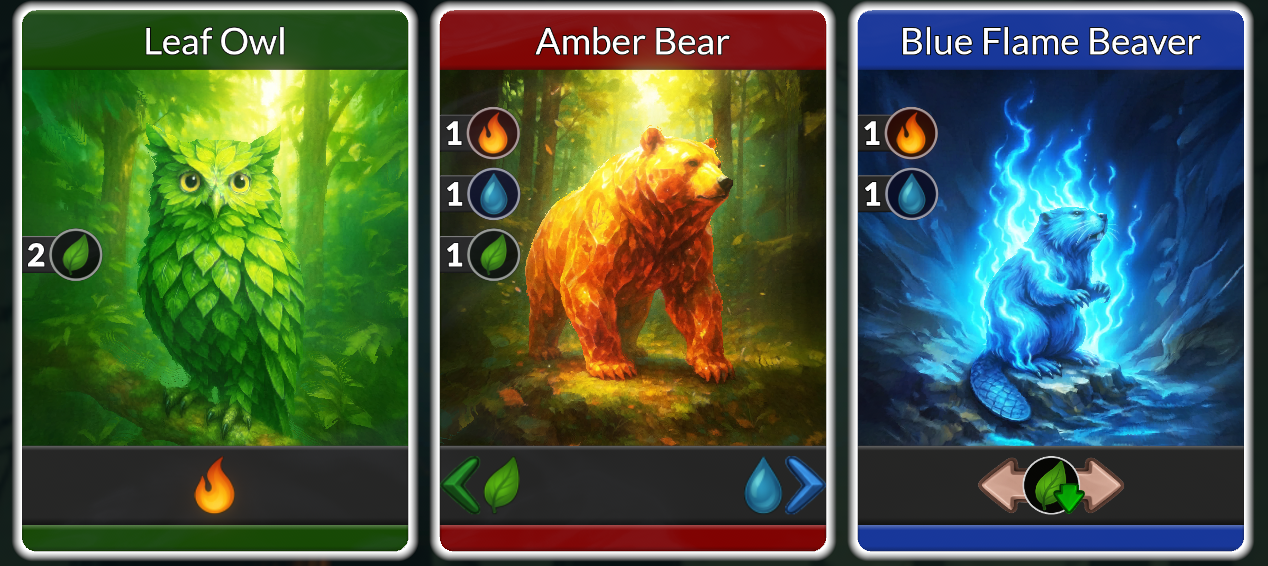
\includegraphics[width=1\linewidth]{img/CoC_e_cards_example.png}
    \caption{Encounter-Karten. Encounter-Karten können grün, rot oder blau sein, eine oder mehrere der Ressourcen Feuer, Wasser und Natur kosten (jeweils links) sowie unterschiedliche Effekte oder Bedingungen haben (jeweils unten).}
    \label{fig:e_card_example}
\end{figure}

\subsubsection{Zauberkarten und Bewegungsfähigkeiten}
Um die Level zu lösen, stehen dem Spieler zusätzlich Zauberkarten zur Verfügung.
Zauber erweitern das durch die Encounter-Karten entstehende Puzzle um eine weitere Ebene, indem sie dem Spieler erlauben, die bestehende Situation gezielt zu beeinflussen.
Ein wichtiger Teil dieser Fähigkeiten verändert die Position der Encounter-Karten, da diese in \coc\ eine zentrale strategische Rolle spielt. 
Unterschiedliche Zauber verfolgen dabei bewusst unterschiedliche Ansätze. 
Beispielweise gibt es Zauberkarten, die zwei benachbarte Karten tauschen oder eine Karte über mehrere andere hinweg verschieben.
Andere Zauber ermöglichen es, einzelne Karten für eine bestimmte Anzahl von Aktionen vollständig aus der Reihe zu entfernen oder eine Karte hinter einen anderen zu \glqq verstecken\grqq, sodass erst das Bezahlen der vorderen Karte die hintere wieder ins Spiel bringt.
Dadurch können Bedingungen auf Encounter-Karten gezielt hergestellt, aufgelöst oder zu einem günstigeren Zeitpunkt aktiviert werden.
Andere Zauber greifen an völlig anderen Stellen in das System ein: Sie können Kartenkosten reduzieren, zusätzliche Ressourcen erzeugen, Karten verwandeln oder duplizieren, Statuseffekte anwenden oder auf bestimmte Karteneigenschaften und bereits vorhandene Synergien reagieren. 
Unterschiedliche Zauber eröffnen dadurch unterschiedliche Lösungswege für dieselbe Spielsituation.
Der eigentliche spielerische Anspruch entsteht somit aus dem Zusammenspiel mehrerer Ebenen: Ressourcenmanagement, Aktionsreihenfolge, Positionierung, Timing, Kartenmechaniken und der strategische Einsatz der eigenen Zauber. 
Ein Level ist dadurch weniger mit einem klassischen Kartenkampf vergleichbar als mit einer dynamischen und strategischen Problemstellung, deren Ausgangszustand durch gezielte Manipulation in eine lösbare Situation überführt werden muss.

\subsubsection{Unterschiede zu Deckbuilding-Spielen}
Der zentrale Gameplay Loop von \coc\ unterscheidet sich von klassischen Deckbuilding-Kartenspielen insbesondere durch den hohen Stellenwert von Vorausplanung, Reihenfolge und Zustandsveränderungen innerhalb eines Levels.
In vielen Deck-building-Spielen besteht ein wesentlicher Teil der Spielerfahrung darin, die aktuell gezogene Kartenhand möglichst effizient zu nutzen.
Nachdem diese ausgespielt wurde, entsteht mit der nächsten Hand eine neue Situation, auf die der Spieler erneut reagieren muss.
Strategische Planung findet zwar statt, wird jedoch fortlaufend durch das Ziehen neuer Karten und damit durch neue, zuvor nicht vollständig bekannte Handlungsmöglichkeiten geprägt.
In \coc\ liegt dagegen ein großer Teil der relevanten Information bereits offen vor dem Spieler. 
Die Encounter-Karten, ihre Kosten, ihre Effekte, ihre Positionen sowie die eigenen verfügbaren Zauber sind bekannt. Dadurch können nicht nur einzelne Aktionen optimiert, sondern ganze Aktionsfolgen im Voraus geplant werden.
Dabei verändert nahezu jede Entscheidung die nachfolgende Spielsituation. 
Wird eine Encounter-Karte bezahlt und aus der Reihe entfernt, rücken die verbleibenden Karten zusammen und bilden neue Nachbarschaften. 
Dadurch können Bedingungen anderer Karten plötzlich erfüllt oder aufgehoben werden. 
Gleichzeitig werden Ressourcen ausgegeben oder durch Karteneffekte zurückgewonnen, Kosten anderer Karten verändert und zeitabhängige Mechaniken um eine weitere Aktion vorangetrieben. 
Auch der Einsatz von Zaubern kann Positionen, Kartenarten, Kosten oder andere Eigenschaften verändern und damit wiederum spätere Aktionen vorbereiten.
Der Spieler muss daher nicht nur entscheiden, welche Aktion aktuell vorteilhaft ist, sondern welche Reihenfolge von Aktionen das Level insgesamt in einen lösbaren Zustand überführt. 
Eine zunächst ungünstige Aktion kann beispielsweise notwendig sein, um Karten zusammenrücken zu lassen, dadurch einen Effekt zu aktivieren, neue Ressourcen zu erhalten und erst mehrere Schritte später eine besonders teure Karte bezahlen zu können.
Der Gameplay Loop ähnelt damit stärker einem strategischen, dynamischen Puzzle mit weitgehend vollständiger Information als einer fortlaufenden Optimierung zufällig entstehender Kartenhände. 
Die Herausforderung entsteht aus dem Zusammenspiel von Ressourcenmanagement, Aktionsreihenfolge, Positionierung, Timing, Kartenmechaniken und Zaubern und ermöglicht dadurch eine wesentlich stärkere Vorausplanung über mehrere miteinander verknüpfte Spielzüge hinweg.

\subsubsection{Zugänglichkeit und Lernkurve}
Trotz seiner strategischen Tiefe soll \coc\ einen sehr zugänglichen Einstieg bieten. 
Das grundlegende Ziel eines Levels ist unmittelbar verständlich: Karten besitzen Kosten in wenigen, klar unterscheidbaren Ressourcen und müssen durch den gezielten Einsatz dieser Ressourcen und der verfügbaren Fähigkeiten aufgelöst werden.
Die Komplexität entsteht erst schrittweise durch zusätzliche Karteneffekte, Bedingungen, Positionierungsregeln, Timing-Mechaniken, Zauber und weitere Systeme. 
Neue Elemente können dadurch auf einem bereits verstandenen Fundament aufbauen, anstatt den Spieler zu Beginn mit der gesamten Systemtiefe gleichzeitig zu konfrontieren.
So soll eine Lernkurve entstehen, bei der der zentrale Gameplay Loop schnell verständlich und spielbar ist, das Spiel jedoch mit zunehmender Erfahrung kontinuierlich neue Zusammenhänge, Interaktionen und strategische Möglichkeiten eröffnet. 
Die langfristige Tiefe entsteht damit nicht aus einem komplizierten Einstieg, sondern aus der schrittweisen Kombination zunächst leicht verständlicher Einzelmechaniken.

\subsubsection{Spielmodi}
Der puzzle-artige Core Gameplay Loop von \coc\ bildet die Grundlage von zwei verschiedenen Spielmodi, dem \textbf{Challenge-Modus} und dem \textbf{Roguelite-Modus}. 
Beide verwenden dieselben grundlegenden Mechaniken, stellen jedoch bewusst unterschiedliche Anforderungen an den Spieler, die auf deutlich unterschiedliche Spielerfahrungen abzielen.

Im \textbf{Challenge-Modus} geht es darum, jeweils alleinstehende, handgefertigte Level (`Challenges') zu verstehen und zu lösen.
Jedes Level bildet eine eigenständige strategische Problemstellung und kann beliebig oft wiederholt werden. 
Der Spieler kann unterschiedliche Ansätze ausprobieren, Zusammenhänge verstehen und so lange experimentieren, bis er eine Lösung findet.
Die Level werden dabei nicht lediglich zunehmend schwieriger, sondern stellen den Spieler immer wieder vor qualitativ neue Fragestellungen und Kombinationen bereits bekannter Mechaniken.
Damit ein besonders schwieriges Level den Spielfortschritt nicht blockiert, können Challenges übersprungen und später erneut gespielt werden. 
Auf Wunsch kann zudem eine Lösung angezeigt werden. 
So können die Puzzle anspruchsvoll bleiben, ohne vorauszusetzen, dass jeder Spieler jede Aufgabe selbstständig lösen muss.

Im \textbf{Roguelite-Modus} werden mehrere Level zu einer zusammenhängenden Reise verbunden, mit dem Ziel, dass der Spieler seine Strategie kontinuierlich weiterentwickelt, seine Zauberfähigkeiten verbessert und sich so zunehmend herausfordernden Levels stellen kann.
Der Roguelite-Modus bildet das Herzstück von \coc\ und wird im folgenden Abschnitt genauer detailliert.

\subsubsection{Level Editor}
Zusätzlich zum Spielen im Roguelite-Modus oder dem Lösen vorgefertigter Challenges soll es auch einen Level-Editor geben, der es Spielern ermöglicht, auf Grundlage der vorhandenen Karten, Zauber und Spielmechaniken eigene Level zu erstellen und anschließend mit anderen Spielern zu teilen.
Für die Erstellung eines Levels können die verfügbaren Encounter- und Zauber-Karten nach Name, Effekten und Kosten gefiltert und gezielt hinzugefügt, umsortiert oder entfernt werden. 
Für jeden einzelnen Zauber kann zudem festgelegt werden, welche Upgrades aktiviert sind. 
% Über Upgrades ist streng genommen hier noch nicht geredet worden.
Dadurch können sowohl einfache Puzzle mit wenigen Mechaniken als auch gezielt auf bestimmte Fähigkeiten, Synergien oder komplexe Interaktionen zugeschnittene Challenges konstruiert werden.
Ein erstelltes Level kann jederzeit direkt im Editor getestet werden. 
Gelingt es dem Ersteller, das Level während eines solchen Tests erfolgreich zu lösen, wird die dabei verwendete Lösung gespeichert und das Level als \glqq lösbar\grqq\ gekennzeichnet. Wird das Level anschließend verändert, beispielsweise durch das Austauschen einer Karte, eine veränderte Reihenfolge oder eine andere Zauberauswahl, so verliert es diese Markierung automatisch und muss erneut erfolgreich getestet werden.
Nur als lösbar verifizierte Level können veröffentlicht und mit der Community geteilt werden. 
Dadurch wird sichergestellt, dass veröffentlichte Challenges zumindest nachweislich eine funktionierende Lösung besitzen, ohne den Spielern vorzugeben, dass dies die einzige oder optimale Lösung sein muss.
Andere Spieler können veröffentlichte Level anschließend herunterladen, spielen und bewerten. 
Auf diese Weise soll langfristig neben den von uns entwickelten Challenges ein zusätzlicher Pool an nutzergenerierten Inhalten entstehen. 
Besonders interessante, kreative oder anspruchsvolle Kombinationen der vorhandenen Mechaniken können so von der Community selbst entdeckt und weitergegeben werden.
Eine frühe Version dieses Editors ist bereits Bestandteil unseres aktuellen Entwicklungsstands und wird intern zur Erstellung eigener Level genutzt. 
Die grundlegende Funktionalität zur Zusammenstellung und Anpassung von Levels ist damit bereits erprobt. 
Im Rahmen der weiteren Entwicklung soll dieses interne Werkzeug zu einem zugänglichen Community-Editor ausgebaut und um Funktionen zum Validieren, Veröffentlichen, Teilen und Bewertung ergänzt werden.
Der Editor erweitert damit nicht nur den Umfang des Spiels, sondern nutzt zugleich die puzzle-artige Struktur des zentralen Gameplay Loops, um langfristig neue Inhalte über die eigentliche Entwicklungsphase hinaus entstehen zu lassen.

    \subsection{Der Roguelite-Modus}
Im Roguelite-Modus werden mehrere Level zu einer zusammenhängenden Reise verbunden.
Jeder \emph{Run}, also jede angetretene Reise, beginnt mit der Auswahl eines Zaubers als Startfähigkeit, sodass sich verschiedene Runs von Anfang an in Hinsicht der angestrebten Strategie und Lösungsansätze unterscheiden können.
Während der Reise entwickelt der Spieler seine Fähigkeiten kontinuierlich durch neue Zauber, Upgrades und Ressourcen weiter, die er als Belohnung für erfolgreich gelöste Level erhält.
Ein Level muss dabei nicht perfekt gelöst werden, um den Run fortzusetzen.
Kann ein Level mit den verbleibenden Ressourcen nicht vollständig gelöst werden, kann der Spieler über eine `Rasten' Aktion zusätzliche Ressourcen erhalten.
Das Rasten reduziert jedoch die für jede Reise begrenzte Zeit-Ressource um 1.
Ein weniger effizient gelöstes Level führt damit nicht zu einem unmittelbaren Scheitern, sondern hat Konsequenzen für den weiteren Verlauf des Runs.
Der Spieler wird nicht nur danach bewertet, ob er eine einzelne Aufgabe lösen kann, sondern danach, wie gut er seine Ressourcen über die gesamte Reise hinweg einsetzt.
Der Run endet, wenn die verfügbare Zeit zum Rasten oder für andere Aktionen innerhalb der Spielwelt ausgegeben wurde.

\subsubsection{Weltkarte und Struktur eines Runs}
Ein Run in Cycle of Cinder führt den Spieler über eine Weltkarte mit verschiedenen Orten und den dazwischenliegenden Reisewegen.
Entscheidet sich der Spieler, von einem Ort zum nächsten zu reisen, wird ein Weg-Encounter ausgelöst, welches die Ereignisse und Hindernisse auf dieser Reise repräsentiert.
Diese Encounter sind allgemeiner gehaltene Level und weniger stark an einen konkreten Ort gebunden.
Am Zielort angekommen können unterschiedliche ortsspezifische Inhalte auftreten.
Dazu gehören beispielsweise Dialoge mit Charakteren, Begegnungen mit Händlern oder andere Interaktionsmöglichkeiten sowie speziell für diesen Ort entwickelte Level.
Anschließend entscheidet der Spieler, welchen Ort er als Nächstes aufsuchen möchte, wodurch erneut eine Reise mit einem Weg-Encounter beginnt.
Auf diese Weise entsteht der grundlegende Rhythmus eines Runs aus Reise, Weg-Encounter, Zielort mit ortsspezifischem Inhalt und schließlich der Wahl des nächsten Ziels.
Die Weltkarte verbindet damit die einzelnen Encounters zu einer nachvollziehbaren Reise und bildet zugleich den Rahmen für Entscheidungen, Story, Charaktere und weitere Spielsysteme.

\subsubsection{Verschiebung des spielerischen Anspruchs}
\todo{Bei diesem Abschnitt bin ich mir nicht so recht sicher. Braucht vlt.\ nochmal etwas Draufschauen.}
Mit dem Wechsel vom Challenge-Modus zum Roguelite-Modus verschiebt sich auch der Schwerpunkt des spielerischen Anspruchs. Während bei einer Challenge die Qualität der Lösung eines einzelnen Puzzles im Mittelpunkt steht, wird im Roguelite zusätzlich relevant, wie gut der Spieler seinen Build über den gesamten Run entwickelt hat. Wie effizient ein Encounter bewältigt werden kann, hängt somit nicht nur von den Entscheidungen innerhalb des Encounters ab, sondern auch von den zuvor gewählten Zaubern, Upgrades und Synergien.
Diese Gewichtung ist ein typisches Gestaltungsmittel von Roguelites und kann je nach Spiel sehr unterschiedlich ausfallen. Ein Extrembeispiel bilden sogenannte Survivor-Likes wie Vampire Survivors, bei denen ein großer Teil der strategischen Tiefe in der Auswahl und Kombination von Fähigkeiten und Upgrades liegt, während die unmittelbaren taktischen Entscheidungen bewusst vergleichsweise einfach gehalten sind.
Cycle of Cinder soll zwischen diesen Polen liegen. Die einzelnen Encounters bleiben eigenständige strategische Herausforderungen, deren gutes Spielen einen wesentlichen Unterschied macht. Gleichzeitig soll ein gut aufgebautes Loadout spürbar belohnt werden und dazu führen können, dass bestimmte Encounters deutlich einfacher oder effizienter zu bewältigen sind. Der Roguelite-Modus verbindet damit die Qualität des situativen Puzzellösens mit der langfristigen Qualität der Build-Entscheidungen.
Aus dieser Designentscheidung ergeben sich unmittelbar die Anforderungen an die prozedurale Generierung der Roguelite-Encounters.

\subsubsection{Upgradesystem}
Zauber bilden den zentralen Werkzeugkasten des Spielers innerhalb eines Levels.
Jeder Zauber besitzt zunächst eine klar definierte Basisfunktion und kann während eines Runs durch \emph{Upgrades} weiterentwickelt werden.
Upgrades werden im Spiel als Belohnungen angeboten und ermöglichen es, die verfügbaren Zauber gezielt zu spezialisieren.
Dabei gibt es sowohl Verbesserungen, die einen Zauber flexibler oder häufiger einsetzbar machen, als auch funktionale Upgrades, die seine Wirkungsweise erweitern oder verändern.
Die Tiefe dieses Systems lässt sich beispielhaft am Zauber \emph{Piercing Shot} zeigen.

In seiner Basisversion reduziert \emph{Piercing Shot} die Kosten einer Karte um eine Ressource, kann jedoch nur auf Karten angewandt werden, die ausschließlich eine einzige Ressourcenart kosten.
Diese Einschränkung macht den Zauber zunächst situativ und verlangt häufig, seine Einsatzbedingung zunächst durch andere Kartenmechaniken oder Fähigkeiten herzustellen.
Im Verlauf eines Runs können unter anderem folgende Upgrades verfügbar werden:
\begin{description}[itemsep=0pt]
    \item[Mehr Ziele:] Piercing Shot kann nun zwei und mit einem weiteren Upgrade bis zu drei Karten gleichzeitig treffen. Die gewählten Karten dürfen unterschiedliche Kosten besitzen, müssen jedoch genau eine gemeinsame Ressourcenart aufweisen.
    \item[Stärkerer Effekt:] Die gemeinsame Ressourcenart wird nicht nur um eins, sondern stärker reduziert.
    \item[Größere räumliche Freiheit:]
     Einschränkungen hinsichtlich der Position oder Nachbarschaft der ausgewählten Karten können aufgehoben werden.
    \item[Cooldown:] Nach einer bestimmten Anzahl von Aktionen wird \emph{Piercing Shot} erneut verfügbar.
    \item[Wiederaufladen:] Durch bestimmte Ereignisse, beispielsweise wenn mehrere Karten einer konkreten Farbe bezahlt wurden, wird \emph{Piercing Shot} erneut verfügbar.
\end{description}

Diese und weitere Upgrades erhöhen nicht lediglich die Stärke des Zaubers.
Sie beeinflussen auch, welche Situationen \emph{Piercing Shot} lösen kann, wie häufig er eingesetzt werden kann, mit welchen Karten er synergiert und welche Entscheidungen der Spieler während eines Levels priorisiert.
Je nach gewählter Kombination kann sich derselbe Basiszauber dadurch zu deutlich unterschiedlichen Varianten entwickeln.
Das Upgrade-System soll auf diese Weise dafür sorgen, dass die Zauberfähigkeiten des Spielers nicht einfach durch erhöhte Zahlenwerte verbessert werden, sondern primär durch neue mechanische Möglichkeiten und zunehmend komplexe Synergien.

%% Folgender Textabschnitt passt aktuell nirgendwo so richtig hin:
% Der Tauschzauber kann beispielsweise zusätzliche Effekte auf den beiden getauschten Karten auslösen, der Verschiebezauber mit den Karten interagieren, über die hinweg verschoben wird, und der Anhebzauber sowohl beim Entfernen von Karten als auch bei deren Rückkehr weitere Effekte auslösen.
% Weitere Bewegungszaubers und eigene Upgrade-Pfade sollen im Verlauf des Spiels freigeschaltet werden und zusätzliche Möglichkeiten eröffnen, die Kartenreihenfolge zu manipulieren.

\subsubsection{Prozedurale Encounter}
Für den Roguelite-Modus von Cycle of Cinder ist ein prozedurales System geplant, das bei jedem Run neue Encounter aus den vorhandenen Karten und Mechaniken erzeugt. Der Anspruch dieses Systems unterscheidet sich dabei bewusst von der Gestaltung der handgefertigten Challenge Encounter.
Ein handcrafted Challenge-Encounter wird gezielt als einzelnes Puzzle entworfen. Dabei werden das verfügbare Loadout und die Encounter Karten Reihe geziehlt aufeinander abgestimmt, um eine möglichst interessante und oftmals anspruchsvolle Problemstellung zu schaffen. Ein solches Puzzle darf bewusst mehrere Versuche erfordern, da der Spieler es beliebig oft wiederholen, verschiedene Ansätze ausprobieren und schrittweise eine Lösung entwickeln kann.
Für den Roguelite-Modus wäre derselbe Anspruch weder notwendig noch wünschenswert. Ein Encounter ist hier nur ein Bestandteil einer längeren Folge von Herausforderungen innerhalb eines Runs. Ein Encounter der so gestaltet ist, dass ein durchschnittlicher Spieler mehrere Versuche benötigt, wäre im Kontext eines Roguelites nicht wünschenswert: Entweder müsste der Spieler mehrfach versuchen dürfen, was in einem Roguelite viel zulange dauern würde und den Fluss zerstören würde, oder die Spieler würden ständig scheitern, was sich schlecht anfühlt.
Hinzu kommt, dass die Qualität und Schwierigkeit eines Encounter-Puzzles stark vom aktuellen Loadout abhängt. Bei einer handgefertigten Challenge kann dieses Loadout bei der Konstruktion des Puzzles berücksichtigt werden. Im Roguelite-Modus trifft dagegen eine große Zahl unterschiedlicher Builds auf prozedural erzeugte Encounters. Eine automatische Anpassung der Encounter an die jeweilige Stärke des Loadouts wäre dabei sogar kontraproduktiv: Ein besonders gutes Loadout soll sich dadurch belohnend anfühlen, dass bestimmte Situationen deutlich leichter zu lösen sind. Umgekehrt soll ein wenig funktionaler Build spürbare Nachteile haben. Würde der Generator besonders starke Builds automatisch mit schwierigeren Encountern ausgleichen, würde die Bedeutung der Build-Entscheidungen belanglos werden.
Der Algorithmus soll deshalb nicht versuchen, automatisch Puzzle auf dem Niveau handgefertigter Challenges zu erzeugen. Sein zentraler Qualitätsanspruch liegt vielmehr in der mechanischen Kohärenz der generierten Encounter. Die Mechaniken der enthaltenen Karten sollen innerhalb der erzeugten Situation grundsätzlich sinnvoll zum Tragen kommen können. Benötigt eine Karte beispielsweise eine gleichartige Nachbarkarte, muss der Encounter mindestens eine weitere entsprechende Karte enthalten. Verlangt eine Mechanik, dass eine Karte zwischen zwei blauen Karten positioniert wird, müssen genügend blaue Karten vorhanden sein, damit diese Bedingung überhaupt hergestellt werden kann. Auch die Verteilung der 3 Ressourcenkosten-Typen muss gut genug zu den durch Encounter Karten erzeugbaren/verringerbaren Ressourcen passen.
Der Generator soll somit sicherstellen, dass aus den kombinierten Karten eine valide und strategisch interessante Spielsituation entstehen kann, ohne für den aktuellen Build eine bestimmte optimale Lösung vorzugeben. Wie leicht oder schwierig diese Situation mit dem jeweils gewählten Loadout zu bewältigen ist, bleibt bewusst Teil des Roguelite-Gameplays. Auf diese Weise können prozedural erzeugte Encounter für hohe Variation und Wiederspielbarkeit sorgen, während gleichzeitig die Relevanz von Loadout-Building, Synergien und langfristigen Entscheidungen innerhalb eines Runs erhalten bleibt.

\subsubsection{Abgrenzung zu vorgefertigten Encounter-Pools}
Viele Roguelites und Roguelite-Kartenspiele erzeugen ihre einzelnen Level oder Begegnungen nicht vollständig prozedural. Stattdessen existieren häufig für unterschiedliche Schwierigkeitsstufen oder Spielphasen Pools aus vorgefertigten Encountern, aus denen während eines Runs zufällig ausgewählt wird. Dadurch entsteht zwar Variation zwischen den Runs, die einzelnen Spielsituationen selbst wurden jedoch zuvor von Hand definiert.
Für \coc\ ist ein weitergehender Ansatz geplant: Der Generator soll Encounter tatsächlich aus ihren einzelnen Karten, Mechaniken und Abhängigkeiten neu zusammensetzen. Ein solches System wäre deutlich flexibler als die Auswahl aus einem festen Pool und könnte mit einer vergleichsweise begrenzten Menge an Karten und Mechaniken eine wesentlich größere Zahl unterschiedlicher Spielsituationen erzeugen. Gerade für ein Spiel, dessen Level stark von Positionierung, Nachbarschaften, Ressourcen und Karteninteraktionen geprägt sind, bietet dieser Ansatz ein großes Potenzial für langfristige Variation und Wiederspielbarkeit.
Die Entwicklung eines solchen Generators stellt entsprechend einen ambitionierteren technischen und gestalterischen Schritt dar. Aufgrund der klar definierbaren Regeln und Abhängigkeiten der Encounter-Karten halten wir diesen Ansatz jedoch für realistisch umsetzbar. Gleichzeitig besteht eine robuste Rückfalloption: Sollte sich im Entwicklungsprozess zeigen, dass eine vollständig prozedurale Generierung nicht in der gewünschten Qualität erreicht werden kann, kann das System auf ausreichend große Pools aus vorgefertigten und validierten Encounter-Konfigurationen zurückgreifen und diese abhängig von Schwierigkeitsgrad und Run-Fortschritt auswählen.
Damit ist die vollständig prozedurale Generierung das angestrebte Ziel, ohne dass die Funktionsfähigkeit des Roguelite-Modus von ihrem Erfolg abhängig ist.

\subsubsection{Belohnungen und Fortschritt innerhalb der Runs}
Nach jedem erfolgreich abgeschlossenen Level wählt der Spieler eine Belohnung aus einer zufälligen Auswahl.
Dadurch entwickelt sich sein Build kontinuierlich über den Verlauf eines Runs weiter.
Die möglichen Belohnungen lassen sich grundsätzlich in vier Kategorien einteilen:
\begin{itemize}
    \item Metaprogressions-Ressourcen, die über den aktuellen Run hinaus erhalten bleiben und anschließend für persistenten Fortschritt und Verbesserungen eingesetzt werden können.
    \item Run-Ressourcen, die unmittelbar den aktuellen Durchlauf unterstützen, beispielsweise Heilung, Gold oder mehr Auswahl bei späteren Belohnungen.
    \item Neue Zauber, mit denen der Spieler neue strategische Möglichkeiten erschließt.
    \item Upgrades bestehender Zauber, durch die bereits gewählte Fähigkeiten weiterentwickelt, spezialisiert oder um zusätzliche Mechaniken und Synergien ergänzt werden.
\end{itemize}

Damit steht der Spieler nach jedem Level vor einer Entscheidung zwischen kurzfristigem Nutzen, langfristigem Fortschritt und der Weiterentwicklung seines aktuellen Builds.
Insbesondere die Wahl neuer Zauber und Upgrades bestimmt, welche Archetypen und Synergien sich innerhalb eines Runs entwickeln und wie gut diese Fähigkeiten mit den folgenden Levels umgehen können.
Über die Dauer eines Runs soll so schrittweise ein immer stärker individualisierter Build entstehen.
Ähnlich wie bei anderen erfolgreichen Roguelites wird die regelmäßige Auswahl von Belohnungen damit zu einem wesentlichen Bestandteil des Spielflusses:
Nicht nur das erfolgreiche Spielen der Level selbst, sondern auch die Entscheidungen zwischen ihnen bestimmen, wie sich ein Run entwickelt.

\subsubsection{Metaprogression über Runs hinweg}
Neben der Entwicklung des eigenen Builds innerhalb eines Runs soll \coc\ eine umfangreiche persistente Metaprogression bieten.
Fortschritt zwischen einzelnen Runs soll dabei auf zwei unterschiedlichen Ebenen stattfinden.
Die erste Ebene umfasst direkte und leicht verständliche Verbesserungen der Ausgangssituation.
Dazu können beispielsweise mehr verfügbare Zeit oder Lebenspunkte, ein höheres Zauberlimit, weitere Upgrade-Slots für einzelne Zauber, bessere Wahrscheinlichkeiten auf hochwertige Belohnungen oder zusätzliche Ressourcen gehören, mit denen angebotene Belohnungen neu ausgewürfelt werden können.
Diese Verbesserungen sorgen dafür, dass der Spieler auch nach einem gescheiterten Run einen dauerhaften Fortschritt wahrnimmt und sich seine Möglichkeiten schrittweise erweitern.
Darüber hinaus ist ein komplexeres System geplant, das sich in seiner Grundidee am Arcana-System von \emph{Hades II} orientiert.
Anstatt alle freigeschalteten Vorteile automatisch gleichzeitig zu aktivieren, stehen dem Spieler verschiedene permanente Modifikatoren zur Auswahl, die vor jedem Run individuell zusammengestellt werden können.
Die verfügbaren Plätze beziehungsweise ein begrenztes Punktebudget verhindern dabei, dass sämtliche Vorteile gleichzeitig genutzt werden.
Dadurch besteht Metaprogression nicht ausschließlich darin, den Spieler mit jedem Run numerisch stärker zu machen.
Neue Freischaltungen erweitern vielmehr auch die Anzahl möglicher Entscheidungen darüber, mit welchen dauerhaften Vorteilen und strategischen Schwerpunkten ein neuer Run begonnen werden soll.
Mit zunehmendem Fortschritt wächst damit nicht nur die Stärke des Spielers, sondern auch die Vielfalt möglicher Ausgangskonfigurationen und Spielweisen.

\subsubsection{Besondere Level}
Um spezielle Situationen im Spiel besonders hervorzuheben und Monotonie zu vermeiden, können einzelne Level um zusätzliche Regeln erweitert oder durch spezielle Boss-Gegner hervorgehoben werden.

\textbf{Zusatzregeln} sind für ein Level geltende Bedingungen wie beispielsweise, die das Lösen erschweren oder erleichtern.

\begin{center}
	\glqq Alle roten Karten kosten eine Feuer Ressource mehr\grqq
\end{center}
oder
\begin{center}
	\glqq Blaue Karten verringern, wenn sie bezahlt werden, die Kosten ihrer Nachbarn um ein Feuer\grqq
\end{center}
Dafür wurde ein modulares System entwickelt, das die normalen Encounter-Regeln um zusätzliche positive und negative Effekte erweitert und dadurch eine hohe Variabilität erzeugt.
Die Besonderheit liegt darin, dass nicht nur unterschiedliche Sonderregeln kombiniert werden können, sondern auch verschiedene Regelmodelle bestimmen, wann und wie diese aktiv sind.
So können beispielsweise gleichzeitig ein positiver und ein negativer Effekt gelten, während unterschiedliche Mechanismen festlegen, welches Effektpaar aktuell aktiv ist.
Ein Wechsel kann etwa nach einer bestimmten Anzahl von Aktionen erfolgen oder davon abhängen, welche Farbe die zuletzt bezahlte Karte hatte.
Die zusätzlichen Regeln können sehr unterschiedliche Aspekte eines Encounters verändern.
Karten bestimmter Farben oder Positionen können beispielsweise teurer oder günstiger werden oder zusätzliche positive beziehungsweise negative Effekte erhalten -- etwa beim Bezahlen Ressourcen stehlen oder die Kosten benachbarter Karten reduzieren.
Durch die Kombination aus unterschiedlichen Effekten, positiven und negativen Regeln sowie verschiedenen Wechselmechanismen kann aus einem modularen System eine große kombinatorische Zahl qualitativ unterschiedlicher Level entstehen, ohne dass für jede Variante vollständig neue Mechaniken entwickelt werden müssen.

\textbf{Boss-Level} hingegen stellen die aufwendigsten und am stärksten individualisierten Encounter des Spiels dar.
Während Zusatzregeln den regulären Gameplay Loop durch neue Regeln und Effekte variieren, können Boss Encounters deutlich weiter gehen und eigene Mechaniken, Regeln sowie alternative Zielbedingungen einführen.
Statt wie gewohnt einfach alle Encounter-Karten spielen zu müssen, könnte die Besonderheit eines Bosss-Levels beispielsweise darin bestehen, dass der Boss Karten innerhalb der Reihe angreift und ihnen Schaden zufügt.
Der Spieler muss dann nicht nur Ressourcen und Kartenmechaniken verwalten, sondern zusätzlich entscheiden, welche Karten zuerst gerettet werden müssen, bevor sie vom Boss zerstört werden.
Dadurch kann ein Encounter beispielsweise zu einem regelrechten Wettrennen werden: Der Spieler versucht, eine bestimmte Anzahl von Karten rechtzeitig zu bezahlen und zu retten, während der Boss parallel versucht, sie durch Schaden zu vernichten.
Boss Encounters können den bekannten Gameplay Loop damit wesentlich stärker verändern als Special Encounters und sollen als besondere Höhepunkte eines Runs jeweils neue strategische Anforderungen stellen.

    \subsection{Spielererfahrung}

\subsubsection{Spielstile}
Die Challenges unterstützen bewusst zwei unterschiedliche Herangehensweisen. 
Spieler können ein Level zunächst analysieren, mögliche Aktionsfolgen gedanklich durchspielen und eine Lösung möglichst weit im Voraus planen. 
Alternativ können sie auch explorativ vorgehen, unmittelbar verschiedene Aktionen ausprobieren und aus deren Auswirkungen lernen. 
Da Challenges beliebig häufig neu gestartet werden können, sind beide Spielweisen gleichermaßen valide und können je nach Präferenz oder Situation miteinander kombiniert werden.
Beide mögliche Spielweisen bleiben auch im Roguelite-Modus erhalten. 
Auch dort kann ein Encounter sorgfältig vorausgeplant werden. 
Es ist aber genauso möglich ihn eher intuitiv aus dem Bauch heraus zu spielen. 
Nicht optimales Spielen führt dabei nicht zu einem kostenlosen Neustart, sondern kann zur Folge haben, dass eine Rast-Aktion erforderlich ist. 
Beide Spielweisen sind in beiden Spielmodi möglich, allerdings belohnt das Roguelite explizit gutes Planen.

\subsubsection{Puzzle Solving als zentrale Spielmotivation}
Problemlösen gehört zu den grundlegenden Motivationen des Spielens. Jesse Schell geht in seiner Definition des Spiels sogar so weit, ein Spiel als „problem-solving activity, approached with a playful attitude“ zu beschreiben. Die Freude daran, Zusammenhänge zu verstehen, eine zunächst schwierige Situation zu durchdringen und schließlich eine Lösung zu finden, bildet entsprechend einen wesentlichen Teil der Spielerfahrung von Cycle of Cinder.
Gleichzeitig reagieren Spieler sehr unterschiedlich auf schwierige Probleme und insbesondere auf wiederholtes Scheitern. Modelle der Goal Orientation unterscheiden beispielsweise im Hinblick auf die Motivation durch Kompetenzerleben zwischen Approach und Avoidance. Vereinfacht bedeutet dies, dass manche Spieler gezielt Situationen suchen, in denen ihre eigene Kompetenz herausgefordert und weiterentwickelt wird, während andere eher vermeiden möchten, mit Situationen konfrontiert zu werden, in denen die Grenzen der eigenen Kompetenz deutlich werden.
Puzzle geben in gewisser Weise ein besonders klares und unmittelbares Feedback über den eigenen Kompetenzstand. Eine Lösung funktioniert oder sie funktioniert nicht. Gerade bei anspruchsvollen Puzzles wird dadurch sehr deutlich erfahrbar, ob die eigene aktuelle Kompetenz ausreicht, um die gestellte Problemstellung zu durchdringen und zu lösen.
Für Spieler mit einer stärkeren Approach-Orientierung kann genau dieses klare Feedback besonders motivierend sein: Die Herausforderung macht sichtbar, dass die eigene Kompetenz noch nicht ausreicht, und erzeugt damit einen konkreten Anlass, sie zu erweitern. Für stärker Avoidance-orientierte Spieler kann dieselbe Klarheit dagegen belastend wirken, weil ein ungelöstes Puzzle sehr unmittelbar die Grenze der eigenen Kompetenz aufzeigt.


Für manche Spieler entsteht ein besonders befriedigendes Erlebnis gerade daraus, zunächst an einer schwierigen Aufgabe zu scheitern, ihre Mechanismen immer besser zu verstehen und sich die Lösung schließlich selbst zu erarbeiten. Für andere kann derselbe langwierige Lösungsprozess dagegen schnell in Frustration umschlagen. Das Design von Cycle of Cinder soll deshalb anspruchsvolles Puzzle Solving ermöglichen, ohne den Fortschritt jedes Spielers zwingend davon abhängig zu machen.

\subsubsection{Challenge-Modus: Herausforderung ohne Sackgasse}
Im Challenge-Modus dürfen einzelne Encounter bewusst anspruchsvoll sein und mehrere Versuche erfordern. Wer die Herausforderung sucht, kann so lange experimentieren und planen, bis die eigene Lösung gefunden ist. Gleichzeitig kann eine Challenge jederzeit übersprungen und später erneut gespielt oder auf Wunsch eine Lösung angezeigt werden.
Damit wird vermieden, dass aus einer interessanten Herausforderung eine dauerhafte Fortschrittsbarriere entsteht. Auch das Anzeigen einer Lösung ist dabei nicht lediglich als „Aufgeben“ zu verstehen: Untersuchungen zu Insight-Problemen zeigen, dass eine präsentierte Lösung insbesondere nach einem zuvor erfolglosen Lösungsversuch selbst ein Aha-Erlebnis und das damit verbundene plötzliche Verständnis auslösen kann.
Roguelite-Modus: Aus Scheitern wird Effizienz
Der Roguelite-Modus löst dasselbe Problem auf eine andere Weise. Hier muss ein Spieler einen Encounter nicht perfekt lösen, um weiterspielen zu können. Wird keine ausreichend effiziente Lösung gefunden, können über die Rest-Action zusätzliche Ressourcen eingesetzt werden. Der Spieler kommt weiter, bezahlt eine weniger gute Lösung jedoch mit einer begrenzten Ressource des Runs – insbesondere mit Zeit.
Dadurch wird aus der binären Frage „Kann ich dieses Puzzle lösen oder nicht?“ eine graduelle Frage: „Wie effizient kann ich diese Situation mit meinem aktuellen Build lösen?“ Ein sehr analytischer Spieler kann weiterhin versuchen, Encounters möglichst optimal vorauszuplanen. Ein stärker intuitiver oder explorativer Spieler kann dagegen ausprobieren, reagieren und bei Bedarf zusätzliche Ressourcen einsetzen.
Auf diese Weise soll der puzzle-artige Gameplay Loop unterschiedliche Präferenzen zulassen, ohne seinen strategischen Anspruch zu verlieren. Spieler, die schwierige Probleme vollständig durchdringen und selbstständig knacken möchten, finden diese Erfahrung insbesondere in den handcrafted Challenges. Im Roguelite-Modus wird dieselbe Fähigkeit zum Problemlösen in einen weniger binären Kontext eingebettet, in dem nicht eine einzelne ungelöste Aufgabe über Erfolg oder Misserfolg entscheidet, sondern die Qualität vieler Entscheidungen über den Verlauf eines gesamten Runs.

\subsubsection{Puzzle geben starkes Feedback}
Puzzle geben ein besonders klares und unmittelbares Feedback über den eigenen Kompetenzstand: Eine Lösung funktioniert oder sie funktioniert nicht. Gerade bei anspruchsvollen Puzzles wird dadurch sehr deutlich erfahrbar, ob die eigene aktuelle Kompetenz ausreicht, um die gestellte Problemstellung zu durchdringen und zu lösen.
Modelle der Goal Orientation unterscheiden im Hinblick auf die Motivation durch Kompetenzerleben unter anderem zwischen Approach und Avoidance. Abstrakt gesprochen suchen manche Spieler gezielt nach Herausforderungen, die ihre Kompetenz ausreizen und ihnen ermöglichen, diese weiterzuentwickeln, während andere eher vermeiden möchten, mit dem Punkt konfrontiert zu werden, an dem ihre aktuelle Kompetenz nicht ausreicht.
Dabei ist für stärker Avoidance-orientierte Spieler nicht zwangsläufig schon ein einzelner Fehler oder ein gescheiterter Lösungsversuch problematisch. Kritischer ist die Situation, über längere Zeit in einem Zustand des Nicht-Lösens festzustecken und keinen erkennbaren Weg zu haben, diesen zu überwinden. Genau hier setzt der Challenge-Modus von Cycle of Cinder an: Encounters können beliebig oft erneut versucht werden, aber auch übersprungen oder ihre Lösung kann auf Wunsch angezeigt werden. Dadurch muss kein Spieler dauerhaft an einer einzelnen Aufgabe festhängen.
Die Möglichkeit unbegrenzter neuer Versuche erfüllt zugleich eine andere Funktion für stärker Approach-orientierte Spieler. Wer eine schwierige Aufgabe gerade deshalb reizvoll findet, weil sie die eigene Kompetenz herausfordert, kann so lange neue Ansätze ausprobieren, bis die Lösung tatsächlich selbst gefunden wurde. Das Spiel unterstützt damit sowohl das Bedürfnis, eine schwierige Herausforderung durch eigene Kompetenz zu überwinden, als auch das Bedürfnis, eine als blockierend empfundene Situation verlassen zu können.

\subsubsection{Roguelite-Struktur als Ausgleich unterschiedlicher Spielstärken}
\todo{
    Andere Option besser?
}
Roguelite-Struktur als Ausgleich unterschiedlicher Spielstärken
Wie schwierig sich ein Spiel für einen Spieler anfühlt, hängt nicht allein von der objektiven Schwierigkeit einer Aufgabe ab. Entscheidend ist vielmehr das Verhältnis zwischen der eigenen Kompetenz und der gestellten Herausforderung. Hinzu kommen weitere Faktoren wie das Feedback des Spiels, die eigenen Erwartungen und der Vergleich mit der bisherigen eigenen Leistung. Ein Spieler kann dieselbe Herausforderung deshalb sehr unterschiedlich wahrnehmen, je nachdem, ob er erwartet hatte, sie problemlos zu bewältigen, ob er bereits zuvor weiter gekommen ist oder ob das Spiel ihm sehr deutlich signalisiert, dass seine aktuelle Kompetenz nicht ausreicht.
Die Roguelite-Struktur von Cycle of Cinder wirkt mehreren dieser Probleme gleichzeitig entgegen. Ein wichtiger Faktor ist, dass der Spieler zu Beginn eines Runs nicht unmittelbar weiß, wie weit er vom endgültigen Ziel entfernt ist oder welchen konkreten Leistungsstand er erreichen müsste, um den gesamten Run erfolgreich abzuschließen. Fortschritt wird zunächst relativ erlebt: Der Spieler erreicht einen neuen Ort, überwindet weitere Encounter, verbessert seinen Build und kommt innerhalb der Reise weiter. Dadurch entsteht weniger häufig die direkte Wahrnehmung, ein zuvor gesetztes Leistungsziel klar verfehlt zu haben.
Gleichzeitig sorgt die persistente Metaprogression dafür, dass sich die Ausgangsbedingungen über mehrere Runs hinweg verbessern und neue strategische Möglichkeiten freigeschaltet werden. Fortschritt entsteht damit nicht ausschließlich dadurch, dass der Spieler selbst schneller lernt oder seine spielerische Kompetenz stark erhöht. Auch Spieler, deren individuelle Lernkurve flacher verläuft, erhalten zunehmend bessere Voraussetzungen und können dadurch im Laufe der Zeit weiter vordringen. Subjektiv entsteht so kontinuierlich das Gefühl von Entwicklung und wachsender Kompetenz, auch wenn dieser Fortschritt teilweise durch das Spielsystem unterstützt wird.
Darüber hinaus reguliert sich die erlebte Schwierigkeit innerhalb eines Runs zu einem gewissen Grad selbst. Solange die Encounter gut zur aktuellen Spielerkompetenz und zum aufgebauten Loadout passen, können sie effizient gelöst werden und der Spieler schreitet schnell voran. Werden die Herausforderungen zunehmend anspruchsvoller, steigt der Ressourcenverbrauch: Es müssen häufiger zusätzliche Ressourcen eingesetzt oder Rest-Actions genutzt werden, wodurch Zeit verloren geht und der Run früher endet. Sehr starke Spieler verbringen entsprechend weniger Zeit mit für sie trivialen Encountern und erreichen schneller schwierigere Bereiche, während weniger erfahrene Spieler länger in einem Schwierigkeitsbereich verbleiben, der ihrer aktuellen Kompetenz entspricht.
Die Roguelite-Struktur erzeugt damit eine Form indirektee dynamische Schwierigkeitsanpassung.

Ein weiterer Vorteil der Roguelite-Struktur ergibt sich aus der inhärenten Varianz des Loadout-Buildings. Welche Zauber und Upgrades während eines Runs angeboten werden, unterliegt bewusst einem gewissen Zufall. Dadurch entstehen Runs, in denen besonders starke Synergien und funktionierende Builds zustande kommen, ebenso wie Runs, in denen das entwickelte Loadout weniger gut funktioniert.
Entscheidend ist dabei, dass sich die Qualität eines Builds sowohl auf das Spielerlebnis als auch auf die Dauer des Runs auswirkt. Gelingt es, ein besonders starkes und gut synergierendes Loadout aufzubauen, lassen sich Encounter effizienter bewältigen, der Spieler kommt weiter und der Run dauert entsprechend länger. Gerade die Runs, in denen die Systeme besonders gut ineinandergreifen und sich der eigene Build besonders befriedigend anfühlt, nehmen damit automatisch einen größeren Anteil der tatsächlichen Spielzeit ein.
Entsteht dagegen durch ungünstige Belohnungen oder weniger gelungene Build-Entscheidungen ein Loadout, das nur schlecht funktioniert, wird dies zwar ebenfalls spürbar, der betreffende Run endet jedoch typischerweise früher. Der Spieler verbringt dadurch vergleichsweise wenig Zeit in einem Zustand, in dem er bereits merkt, dass sein aktueller Build nicht überzeugend funktioniert, und kann zeitnah mit einem neuen Run und neuen Möglichkeiten beginnen.
Die Run-Struktur erzeugt damit eine günstige zeitliche Gewichtung der durch Zufall und Build-Entscheidungen entstehenden Varianz: Je besser ein Build funktioniert und je befriedigender sich ein Run dadurch anfühlt, desto länger dauert er tendenziell; schwächere Runs verkürzen sich dagegen selbst. Dadurch verbringt der Spieler über die gesamte Spielzeit hinweg überproportional viel Zeit mit den besonders gelungenen und motivierenden Runs.

Auf diese Weise verbindet der Roguelite-Modus unterschiedliche Formen von Fortschritt: Der Spieler kann selbst besser werden, sein Build kann stärker werden und die persistente Metaprogression kann seine zukünftigen Ausgangsbedingungen verbessern. Dadurch können Spieler mit sehr unterschiedlichem Kompetenzniveau über längere Zeit in einem Bereich spielen, der für sie herausfordernd, aber nicht dauerhaft blockierend ist, während gleichzeitig das Gefühl erhalten bleibt, aus eigener Kraft immer weiter in das Spiel vorzudringen.
    \subsection{Thematische Einbettung}

\coc\ bettet seine Mechaniken und sein Gameplay in einen immersiven thematischen Kontext und verfügt über eine Story, welche der Spieler im Laufe des Spiels erlebt. 
Das Spiel ist in einer bereits vor einiger Zeit selbst entwickelten Classic-Fantasy-Welt angesiedelt, deren Geschichte mehrere Zeitalter umfasst. 
Die zentralen Spielelemente besitzen dabei nicht nur eine mechanische Funktion, sondern zugleich einen nachvollziehbaren Platz innerhalb dieser Welt. 
Die Level, die der Spieler bewältigt, stellen konkrete Begegnungen, Aufgaben oder Situationen dar, auf die er während seiner Reise trifft. 
Diese können sowohl an bestimmten Orten stattfinden als auch auf dem Weg von einem Ort zum nächsten. 
Die bereisten Orte besitzen einen konkreten Platz und eine Funktion innerhalb der Spielwelt. 
Sie sind auf einer Weltkarte dargestellt und haben thematisch dazu passende Hintergründe während des Levels.
\todo{
    Hier könnte sich evtl. ein Bild anbieten.
}
Auch die eingesetzten Fähigkeiten sind innerhalb der Spielwelt verankert. Sie stellen Zauber dar, die der Spieler beispielsweise von bestimmten Lehrmeistern erlernt und im Verlauf seiner Reise weiterentwickelt. 
Ebenso sind die Charaktere, denen der Spieler begegnet und mit denen er Dialoge führt, in der Geschichte und Struktur dieser Welt plausibel verortet. 
Auf diese Weise soll nicht lediglich eine thematische Kulisse für die Spielmechaniken entstehen. 
Vielmehr soll der Spieler nach und nach ein tatsächliches Verständnis dafür entwickeln, wo er sich befindet, welchen Weg er zurücklegt, wem er begegnet, welche Bedeutung diese Personen und Orte besitzen und weshalb die einzelnen Spielelemente innerhalb dieser Welt existieren.

\todo{Ich bin von `Zeit-Ressource' als Formulierung nach wie vor nicht überzeugt. Vlt. finde ich was Besseres.}

Eine besondere Rolle spielt dabei die Zeit-Ressource, welche der Spieler insbesondere beim \emph{Rasten} innerhalb der Level ausgibt. 
Sie ist sowohl eine zentrale mechanisch-strategische Ressource als auch ein konkreter Bestandteil der Spielwelt. 
Die während eines Levels ausgegebene Zeit stellt dar, wie lange eine Reise zwischen zwei Orten dauert, wie viel Zeit eine Begegnung beansprucht oder wie lange sich die Spielfigur an einem bestimmten Ort aufhält. 
Die Bewegung durch die Spielwelt, das Bewältigen von Levels sowie die Entscheidung, welche Ziele innerhalb eines Runs verfolgt werden, sind damit unmittelbar mit dem verfügbaren Zeitkontingent verbunden. 
Zeit ist folglich nicht lediglich ein abstrakter Zähler oder eine künstliche Begrenzung des Spielsystems, sondern entspricht thematisch der Zeit, die auch innerhalb der Reise der Spielfigur tatsächlich vergeht.

Die Rahmenhandlung erklärt darüber hinaus zentrale Bestandteile der Roguelite-Struktur selbst. 
Insbesondere wird narrativ begründet, weshalb ein Scheitern nicht das endgültige Ende der Reise darstellt, sondern zu einem erneuten Beginn führt.
Die Spielfigur befindet sich innerhalb eines durch die Handlung etablierten Zeitkreislaufs und verfügt in jedem Run nur über ein begrenztes Zeitkontingent, bevor sie an einen Ausgangspunkt -- einen bestimmten Zeitpunkt innerhalb der Handlung -- zurückversetzt wird. 
Im Verlauf des Spiels kann dieses Zeitkontingent erweitert werden. 
Wiederholte Runs, Scheitern, erneute Versuche und der Umgang mit begrenzter Zeit existieren dadurch nicht nur als abstraktes mechanisches Konstrukt, sondern besitzen eine thematisch nachvollziehbare Bedeutung.

Die inhaltliche und thematische Einbettung wird durch die visuelle Präsentation des Spiels unterstützt. Unterschiedliche Orte, Figuren, Levels, Karten und magische Elemente sollen nicht lediglich als funktionale Oberfläche der Spielmechaniken dienen, sondern die Fantasy-welt gestalterisch vermitteln und ihre jeweiligen Charakteristika sichtbar machen. Die visuelle Gestaltung soll dabei helfen, die Immersion zu fördern und die Welt für den Spieler zum Leben zu erwecken. 
Handlung, Weltgestaltung und visuelle Darstellung ergänzen einander somit und können gemeinsam ein verständlicheres und immersiveres Spielerlebnis schaffen, ohne die Übersichtlichkeit und Lesbarkeit des strategischen Kartenspiels zu beeinträchtigen, sondern es zugänglicher und intuitiver zu gestalten.
Die thematische und narrative Ebene ist dabei bewusst kein Ersatz für die mechanische Motivation und nicht der Hauptfokus des Spiels. 
Die grundlegende Spielerfahrung soll bereits durch die strategischen Systeme, das Lösen schwieriger Spielsituationen und die Entwicklung unterschiedlicher Strategien tragen. 
Spielwelt, Geschichte und visuelle Präsentation ergänzen diese Erfahrung jedoch um Bedeutung, Perspektive und Dringlichkeit: Spieler bewältigen eine Herausforderung zum einen, weil deren Lösung spielerisch befriedigend ist, zugleich aber auch, weil sie verstehen, was diese Herausforderung innerhalb der Welt bedeutet und welchem übergeordneten Ziel sie dadurch näherkommen.

\subsubsection{Lore und Handlung}
Die Welt von \coc\ verfügt über eine umfangreichere, mehrere Zeitalter umfassende Hintergrundgeschichte. 
Die folgende Darstellung beschränkt sich bewusst auf die für das Spiel unmittelbar relevanten Zusammenhänge. Die Welt ist darüber hinaus als langfristiger erzählerischer Rahmen angelegt, in dem perspektivisch auch weitere Spiele angesiedelt werden können.
In einem früheren Zeitalter waren die verschiedenen Völker der Welt von Konflikten geprägt. Magie war zu dieser Zeit kaum zugänglich und konnte im Wesentlichen nur von einem Elfenvolk genutzt werden, dessen gewaltiger Baum des Lebens als Quelle magischer Energie diente. Durch die Zusammenarbeit von Wissenschaftlern und Zwergen wurde schließlich entdeckt, dass bestimmte Edelsteine diese Energie speichern können. Auf dieser Grundlage entstand eine Art magischer Kompass, mit dessen Hilfe weitere, bis dahin nicht nutzbare Magievorkommen auf der Welt lokalisiert wurden.
Um diese Quellen zugänglich zu machen, schlossen sich zuvor verfeindete Völker zusammen und pflanzten an den entsprechenden Orten Setzlinge des Baums des Lebens. Aus ihnen entstanden neue magische Bäume, die nach und nach ein weltumspannendes Netz bildeten und Magie für große Teile der Bevölkerung verfügbar machten.
Im folgenden Zeitalter wurde Magie systematisch erforscht, gelehrt und zunehmend in den Alltag der verschiedenen Völker integriert. Es entstanden bedeutende Zentren magischer Forschung und Ausbildung. An ihrer Spitze stehen die Great Sages, die mächtigsten Magier ihrer jeweiligen Disziplin und zugleich zentrale Autoritäten dieser neuen magischen Ordnung.
Zu Beginn von Cycle of Cinder tritt die Spielfigur bei einem dieser Great Sages in die Lehre: einem Magier, der für seine Beherrschung der Zeit bekannt ist. Bereits während der Ausbildung wird Zeitmanipulation als Bestandteil der Welt und der Magie etabliert. So können beispielsweise Trainingssituationen wiederholt werden, indem der Meister die Zeit um einen kurzen Zeitraum zurücksetzt.
Kurz darauf werden Meister und Schüler von einer fremden Entität angegriffen. Dabei erfährt der Spieler, dass zeitgleich auch die übrigen Great Sages ausgeschaltet werden sollen. Ziel dieses koordinierten Angriffs ist es, den wichtigsten Widerstand gegen eine bevorstehende Invasion aus einer parallel existierenden Welt zu beseitigen – jener Welt, aus der die Magie ursprünglich stammt und in der dämonische Wesen leben.
Um seinem Schüler eine Möglichkeit zu geben, diese Ereignisse noch zu verhindern, setzt der Meister einen uralten Zauber ein. Dabei opfert er sich selbst, zerfällt zu Asche und bindet den Spieler an einen Zeitkreislauf: den namensgebenden Cycle of Cinder.
Von diesem Moment an hat der Spieler innerhalb jedes Runs nur ein begrenztes Zeitkontingent, um die Great Sages zu finden und zu retten. Läuft diese Zeit ab oder scheitert der Spieler, wird er an einen früheren Zeitpunkt zurückversetzt und beginnt den Versuch erneut. Im Verlauf des Spiels kann der Spieler seine Möglichkeiten innerhalb dieses Kreislaufs erweitern und unter anderem mehr Zeit für zukünftige Runs gewinnen.
Damit erklärt die Rahmenhandlung unmittelbar zentrale Roguelite-Mechaniken des Spiels: das wiederholte Beginnen eines Runs, das Fortbestehen von Wissen und Fortschritt über mehrere Versuche hinweg sowie Zeit als zentrale Ressource sind nicht nur abstrakte Spielregeln, sondern ergeben sich direkt aus der Handlung und der Logik der Spielwelt.

    \subsection{Projektplan}

\todo{Better title; Introductory sentence}

\subsubsection{Marktsituation}

Singleplayer-Kartenspiele und rundenbasierte Roguelites haben sich in den vergangenen Jahren als etabliertes und wirtschaftlich relevantes Segment des Indie-Computerspielmarktes entwickelt.
Insbesondere Spiele, die strategische Entscheidungen mit einer Run-basierten Struktur, wechselnden Spielstrategien und hoher Wiederspielbarkeit verbinden, haben eine große und langfristig aktive Zielgruppe hervorgebracht.

Das hohe Marktpotenzial dieses Segments zeigen zunächst einige außergewöhnlich erfolgreiche Vertreter.
Einer der frühen und genreprägenden Titel ist \emph{Slay the Spire}, das bereits 2019 mehr als 1,5 Millionen verkaufte Einheiten erreicht hatte.
In den folgenden Jahren haben weitere Spiele gezeigt, dass dabei nicht nur direkte Nachfolger dieses Spielprinzips erfolgreich sein können.
\emph{Inscryption} verband Kartenspielmechaniken mit Puzzle-, Horror- und narrativen Elementen und wurde innerhalb von weniger als drei Monaten mehr als eine Million Mal gekauft.
\emph{Balatro} interpretierte das strategische Singleplayer-Kartenspiel erneut auf grundlegend andere Weise und erreichte innerhalb seines ersten Jahres mehr als fünf Millionen Verkäufe.
Dass das Interesse an diesem Marktsegment weiterhin sehr hoch ist, zeigt zuletzt \emph{Slay the Spire 2}: Bereits in der ersten Woche seines Early-Access-Starts im März 2026 wurden drei Millionen Exemplare verkauft und mehr als 25 Millionen Runs gespielt.

Diese außergewöhnlichen Millionenerfolge bilden jedoch nur die besonders sichtbare Spitze eines deutlich breiteren Marktes.
Neben ihnen existiert eine große Zahl kleinerer und mittlerer Produktionen im Bereich der Singleplayer-Kartenspiele und rundenbasierten Roguelites, die innerhalb des Genres eine stabile Zielgruppe erreichen und wirtschaftlich erfolgreich sind.
Der Markt wird damit nicht allein von einzelnen Ausnahmeerscheinungen getragen, sondern von einer etablierten Spielerschaft mit kontinuierlichem Intereasse an neuen Titeln und neuen Interpretationen dieser Spielprinzipien.

Gerade die Vielfalt erfolgreicher Spiele innerhalb dieses Umfelds ist für \coc\ relevant.
Titel wie \emph{Slay the Spire} stehen für klassisches Deckbuilding, während \emph{Balatro} oder \emph{Inscryption} zeigen, dass sich dieselbe grundsätzliche Zielgruppe auch mit deutlich anderen Karten- und Spielsystemen erreichen lässt.
Gleichzeitig demonstrieren Roguelites wie \emph{Hades} oder \emph{Shogun Showdown} die Attraktivität eines anderen Ansatzes zur Entwicklung der Spielstrategie: Spieler ziehen ihre Handlungsmöglichkeiten nicht fortlaufend zufällig aus einem Deck, sondern stellen während eines Runs gezielt eine Auswahl an Fähigkeiten, Verbesserungen und Synergien zusammen.
% Das ist jetzt nicht so richtig ein *Gegensatz*, dass passiert in Deckbuildern halt auf der höheren Ebene.
% Insbesondere ist zu sagen (aber nicht hier in diesem Antrag), dass ein Roguelite ohne RNG in den Upgrades halt auch total lame ist, weil man dann doch einfach das gleiche wieder spielt.

\coc\ liegt an der Schnittstelle dieser Zielgruppen.
Das Spiel richtet sich insbesondere an Spieler strategischer Singleplayer-Kartenspiele und rundenbasierter Roguelites, spricht durch sein Loadout-Building aber ebenso Spieler an, die aus anderen Roguelites die gezielte Entwicklung individueller Archetypen oder Synergien kennen.
Durch den puzzle-artigen Gameplay Loop kommt zusätzlich eine Zielgruppe hinzu, die Freude daran hat, komplexe Spielsituationen zu analysieren, Zusammenhänge zu erkennen und konkrete Lösungswege zu entwickeln.

Eine weitere angrenzende Zielgruppe bilden Spieler etablierter digitaler und analoger Strategie- und Kartenspiele wie \emph{Magic: The Gathering}, \emph{Magic Arena} oder \emph{Hearthstone}.
Die Größenordnung dieses Marktes zeigt sich unter anderem an mehr als 50 Millionen \emph{Magic}-Spielern seit Bestehen der Marke und über zehn Millionen registrierten Spielern von \emph{Magic Arena}.
Auch \emph{Hearthstone} hatte bereits 2018 mehr als 100 Millionen Spieler erreicht.
Diese Spiele unterscheiden sich strukturell deutlich von \coc, sprechen jedoch ebenfalls Spieler an, die Freude am Entdecken und Verstehen komplexer Interaktionen, Kombinationen und Synergien sowie am Aufbau eigener strategischer Spielweisen haben.
Entsprechend gehören auch Spieler moderner strategischer Brett- und Kartenspiele zur erweiterten potenziellen Zielgruppe.

Damit bewegt sich \coc\ in einem bereits etablierten und nachweislich wirtschaftlich attraktiven Markt, ohne ausschließlich von der Zielgruppe eines einzelnen Vergleichstitels abhängig zu sein.
Gleichzeitig zeigt die Bandbreite erfolgreicher Spiele innerhalb dieses Umfelds, dass sich neue Spielkonzepte durch eine klare mechanische Eigenständigkeit innerhalb des Genres positionieren können.

\subsubsection{Unique Selling Points}

\coc\ unterscheidet sich von bisher im Genre etablierten Spielen insbesondere durch folgende Eigenschaften.

\paragraph{Neu entwickelter, eigenständiger Gameplay Loop}
Cycle of Cinder basiert auf einem von uns neu entwickelten, Encounter-basierten Spielprinzip, das sich deutlich von klassischen Kartenkampf- und Deckbuilding-Systemen unterscheidet.

\paragraph{Puzzle-Gameplay mit hoher Player Agency}
Der Spieler löst strategische Problemsituationen mit direkt verfügbaren Fähigkeiten. Der Fokus liegt damit stärker auf Planung, Verständnis und der gezielten Anwendung der eigenen Werkzeuge als auf der Optimierung zufällig gezogener Handkarten.

\paragraph{Ein Core Gameplay Loop, der auch ohne Roguelite-Struktur trägt}
Der zentrale Gameplay Loop funktioniert bereits als eigenständiges Puzzle-Spiel. Im Challenge-Modus wird er in handgefertigten Aufgaben gezielt auf einzelne Mechaniken und Problemstellungen fokussiert. Der Roguelite-Modus erweitert denselben Kern um Build-Entwicklung, Progression und prozedurale Variation. Dadurch entstehen zwei klar voneinander unterscheidbare Spielerlebnisse auf Basis desselben grundlegenden Systems.

\paragraph{Loadout-Building statt klassischem Deckbuilding}
Während eines Runs stellt der Spieler ein Loadout aus Zaubern und Upgrades zusammen, die in den Encountern direkt verfügbar sind. Dadurch bleiben Build-Entscheidungen langfristig relevant und der Zufallseinfluss innerhalb der einzelnen Spielsituationen wird reduziert.

\paragraph{Qualitativ tiefgreifende Upgrade-Systeme}
Upgrades erhöhen nicht lediglich Werte, sondern verändern die Funktionsweise von Fähigkeiten, eröffnen neue Interaktionen und ermöglichen unterschiedliche Spezialisierungen, Synergien und Archetypen.

\paragraph{Roguelite mit prozedural generierten Puzzle-Encountern}
Das Herzstück des Spiels verbindet den puzzle-artigen Gameplay Loop mit prozedural erzeugten Herausforderungen, Run-basierter Build-Entwicklung und persistenter Metaprogression.

\paragraph{Handgefertigter Challenge-Modus}
Zusätzlich zum Roguelite-Modus bietet das Spiel gezielt entwickelte Puzzle-Challenges, in denen jeder Encounter eine qualitativ neue spielerische Fragestellung in den Mittelpunkt stellt.

\paragraph{Community Editor und nutzergenerierte Inhalte}
Spieler können eigene Encounters erstellen und über Steam mit der Community teilen. Dadurch kann der Puzzle-Charakter des Spiels langfristig durch neue, von Spielern entwickelte Herausforderungen erweitert werden.

\paragraph{Fantasy-Welt und fortlaufende Geschichte}
Gameplay, Progression und Encounters sind in eine eigenständige Fantasy-Welt mit Lore, Worldbuilding und einer fortlaufenden Handlung eingebettet.

\subsubsection{Aktueller Entwicklungsstand}
\coc\ ist konzeptionell bereits weit fortgeschritten.
Die grundlegenden Spielsysteme, die Roguelite-Struktur, zentrale Progressionsmechaniken sowie die Spielwelt, ihre Geschichte und die grobe narrative Handlung sind in ihren wesentlichen Grundzügen ausgearbeitet.
Der Schwerpunkt der bisherigen praktischen Entwicklung lag zunächst bewusst auf dem neu entwickelten Gameplay Loop mit puzzle-artigen Levels.
Hierfür wurde ein spielbarer Proof of Concept entwickelt, mit dem sich bereits unabhängig von den späteren Roguelite-Systemen überprüfen lässt, ob das grundlegende Gameplay funktioniert, verständlich ist und Spielern dauerhaft Freude bereitet.
Dieser Schritt war aus unserer Sicht notwendig, bevor weitere Systeme aufgesetzt werden: Die Roguelite-Struktur soll nicht einen noch unbewiesenen Gameplay-Kern interessant machen müssen, sondern auf einem bereits funktionierenden und eigenständig tragfähigen Fundament aufbauen.
Der bestehende Proof of Concept umfasst neben der funktionalen Umsetzung der zentralen Mechaniken bereits eine visuelle Gestaltung, die in wesentlichen Teilen nahe an der für das fertige Spiel angestrebten Präsentation liegt. Damit können neben der grundsätzlichen Funktionsweise des Gameplay Loops bereits heute auch Spielgefühl, Lesbarkeit und visuelle Wirkung unter realistischen Bedingungen getestet werden.

\todo{
	Link zur Demo !!!
}

\subsubsection{Nächster Entwicklungsschritt}
Der nächste wesentliche Entwicklungsschritt besteht darin, das bislang vor allem auf einzelne Level fokussierte Gameplay in einen zunächst vereinfachten Roguelite-Modus zu überführen.
Dadurch sollen erstmals mehrere Level zu einem vollständigen Run verbunden und die zentralen Systeme des späteren Roguelite-Erlebnisses gemeinsam getestet werden.
Dabei müssen insbesondere grundlegende Fragen des Game Balancing und der zeitlichen Struktur beantwortet werden:
Wie viele Level sollte ein Run umfassen? Wie lange sollte ein durchschnittlicher Run dauern? In welchen Abständen benötigt der Spieler Belohnungen? Wie häufig sollten neue Zauber angeboten werden und wie häufig Upgrades bestehender Fähigkeiten? Wie schnell soll sich ein Build innerhalb eines Runs entwickeln und ab welchem Zeitpunkt sollen deutliche Synergien und Archetypen entstehen?
Diese Fragen lassen sich nur eingeschränkt isoliert beantworten. Sie müssen im Zusammenspiel innerhalb eines tatsächlich spielbaren Roguelite-Modus getestet und iterativ angepasst werden.
Auf dieser Basis können anschließend weitere Systeme wie die persistente Metaprogression und die vollständige narrative Einbettung aufgebaut werden.

\subsubsection{Ziel des geförderten Prototyps}
Ziel der Prototypenentwicklung ist eine authentische, spielbare Version von \coc, die den Spielern bereits einen repräsentativen Eindruck davon vermittelt, wie sich das spätere vollständige Spiel anfühlen wird.
Der Prototyp soll daher nicht lediglich einzelne technische Systeme demonstrieren, sondern den neu entwickelten Gameplay-Loop erstmals innerhalb eines zusammenhängenden Roguelite-Erlebnisses spielbar machen.
Dafür soll insbesondere ein Ausschnitt des Roguelite-Modus entstehen, in dem mehrere Level zu einem Run verbunden werden und der Spieler seine Strategie durch neue Zauber und Upgrades kontinuierlich weiterentwickelt.
Gleichzeitig soll die narrative und thematische Einbettung bereits so weit umgesetzt werden, dass Spielwelt, Charaktere und Handlung erkennbar werden und Spieler einschätzen können, welche Rolle diese Elemente im späteren Gesamtprodukt einnehmen.
Der Prototyp ist damit zugleich ein wichtiger Entwicklungsschritt und ein Instrument zur externen Validierung.
Er soll vor dem geplanten Early Access Release unter anderem im Rahmen einer Kickstarter-Kampagne und eines Steam Next Fests öffentlich spielbar gemacht werden.
Potenzielle Spieler sollen das Spiel nicht nur anhand von Beschreibungen, Screenshots oder Videos beurteilen können, sondern selbst erfahren, wie sich der neue Gameplay Loop, die Roguelite-Struktur, das Loadout-Building und die narrative Einbettung zu einem vollständigen Spielerlebnis verbinden.
Das Ziel ist damit ausdrücklich kein isolierter Technologie-Demonstrator, sondern ein repräsentativer Prototyp des späteren Spielerlebnisses, auf dessen Grundlage sowohl das weitere Game Design als auch Balancing, Inhalte und Präsentation bis zum Early Access gezielt weiterentwickelt werden können.


\end{document}
